\documentclass[a4,10pt]{article}

\usepackage[utf8]{inputenc}
\usepackage[english,spanish]{babel}
\usepackage{verbatim}
\usepackage{graphicx}
\usepackage{amsmath}
\usepackage{hyperref}

\begin{document}

\title{Aplicaciones de Geometría Proyectiva}
\author{Gustavo Quesada Menchón}
\date{}
\maketitle
\newpage

\tableofcontents
\newpage

\section{Introducción}

Este documento va ha tratar sobre geometría proyectiva y sus aplicaciones, de cómo con sus operaciones básicas nos facilita la tarea en aplicaciones como el tratamiento de imágenes, reconocimiento facial, visión estereoscópica, etc. Para abordar el tema, se va dividir en varias partes. Una pequeña introducción con un poco de historia, definiciones y conceptos básicos sobre geometría proyectiva. Una segunda parte donde se explican un poco las principales operaciones/transformaciones que nos pueden ser útiles. Una tercera parte donde se profundiza algo más en técnicas aplicadas en el tratamiento de imágenes 3D que se ha utilizado en algunos proyectos, y una parte final, con un pequeño resumen y conclusiones sobre el tema.


%%%%%%%%%%%%%%%%%%%%%%%%%%%%%%%%%%%%%%%%%%%%%%%%%%%%%%%%%%%%%%%%%%%%%%
\section {Definición y conceptos básicos}

Para comenzar explicando qué es la geometría proyectiva, veamos un poco de historia:

\emph{“
Gérard Desargues es el iniciador de la geometría proyectiva, pues fundamentó matemáticamente los métodos de la perspectiva que habían desarrollado los artistas del Renacimiento, y aunque su trabajo fue publicado en 1639, pasó desapercibido durante dos siglos (excepto dos teoremas), ensombrecido por la influyente obra de Descartes.\\
En el siglo XIX, la geometría proyectiva y la geometría hiperbólica, se establecieron dentro de las matemáticas, pero lo que acabó de enraizarlas, posiblemente, fue hallar un modelo analítico. Dentro del contexto de la geometría euclidiana-cartesiana se puede construir la geometría proyectiva, y si se acepta la primera, hay que admitir la segunda. Este proceso finalizó definitivamente a principios del siglo XX, pues Einstein, apoyándose en los exhaustivos desarrollos geométricos de los matemáticos del siglo XIX, consiguió demostrar que, a gran escala, el universo se puede interpretar mejor con estas nuevas geometrías que con el rígido espacio euclidiano.”}\\%poner por aqui una referencia
\\
Se podría decir que este interés por desarrollar la geometría proyectiva se debe al cambio en la temática de la pintura, ya que surge de la preocupación del artista de representar el mundo tridimensional en su lienzo bidimensional. En el periodo medieval las pinturas eran de carácter principalmente religioso y los pintores representaban a los personajes y objetos de una forma sumamente estilizada, generalmente sobre fondo dorado, para subrayar que el cuadro no tenía conexión con el mundo real. En el Renacimiento con la llegada del humanismo y el antropocentrismo la pintura se centra en la representación del mundo real.

Una vez establecidos los orígenes, podemos dar alguna definición breve:\\
\emph{
Se llama geometría proyectiva a la rama de la matemática que estudia las propiedades de incidencia de las figuras geométricas, pero abstrayéndose totalmente del concepto de medida.}\\

La geometría proyectiva puede entenderse, informalmente, como la geometría que se obtiene cuando nos colocamos en un punto, mirando desde ese punto. Esto es, cualquier línea que incide en nuestro ojo nos parece ser sólo un punto, en el Plano proyectivo, ya que el ojo no puede ver los puntos que hay detrás.
De esta forma, la geometría proyectiva también equivale a la proyección sobre un plano de un subconjunto del espacio en la geometría euclidiana tridimensional. Las rectas que salen del ojo del observador se proyectan sobre puntos. Los planos definidos por cada par de ellas se proyectan sobre rectas.

La geometría proyectiva también es aquella que trata las propiedades que se conservan bajo proyecciones. Tiene aplicaciones en visión artificial, funcionamiento de cámaras, reconstrucción de imágenes bidimensionales en tres dimensiones, etc. En resumen es la geometría asociada al modo en que el ojo humano percibe el mundo.

\section{Propiedades, operaciones y transformaciones más usadas}

Vamos a tratar en este apartado las transformaciones relacionadas con el tratamiento de imágenes en 3D. Para ello también será necesario explicar alguna de las ventajas que nos ofrece la geometría proyectiva.\\
\begin{enumerate}

\item \textbf{Transformaciones proyectivas 3D}\\
En las transformaciones geométricas de un sistema cartesiano 3D, un punto en el espacio se define por las coordenadas (X, Y, Z) y un pixel en la imagen por el par de coordenadas (x, y).
A continuación se presentan las transformaciones geométricas 3D fundamentales para el tratamiento de imágenes en tres dimensiones, la rotación y traslación. 
En la figura (Fig. \ref{fig:fig1})se presenta un sistema de coordenadas 3D (X, Y, Z) que ha sufrido una transformación de translación y rotación. El sistema nuevo generado como resultado de dicha transformación es el definido por (X’, Y ’, Z’). La ecuación que relaciona ambos sistemas de coordenadas es la siguiente: 

\begin{equation}
\begin{pmatrix}
X'\\
Y'\\
Z'
\end{pmatrix}
= R
\begin{pmatrix}
X\\
Y\\
Z
\end{pmatrix}
+ t
\end{equation}

donde t es un vector 3 x 1 que identifica la translación y R es una matriz 3 x 3 que representa la rotación del sistema de coordenadas.

\underline{Rotación}\\
En el escenario 3D, la matriz R se define de manera particular para cada uno de los ejes. De esta manera, una transformación de rotación se descompone en tres subrotaciones:\\
\begin{equation}
R_Z =
\begin{bmatrix}
\cos(\omega Z) & \sin(\omega Z) & 0\\
-\sin(\omega Z) & \cos(\omega Z) & 0\\
0 & 0 & 1\\
\end{bmatrix}
\end{equation}
\begin{equation}
R_Y =
\begin{bmatrix}
\cos(\omega Y) & \sin(\omega Y) & 0\\
0 & 1 & 0\\
\sin(\omega Y) & 0 & \cos(\omega Y)\\
\end{bmatrix}
\end{equation}
\begin{equation}
R_X =
\begin{bmatrix}
1 & 0 & 0\\
0 & \cos(\omega X) & \sin(\omega X)\\
0 & -\sin(\omega X) & \cos(\omega X)\\

\end{bmatrix}
\end{equation}

Como se trata de aplicaciones lineales, las tres rotaciones pueden combinarse formando una única expresión de rotación global. Matemáticamente se expresa como la multiplicación de todas ellas.\\
\begin{equation}
R (\omega X , \omega Y , \omega Z ) = R_X (\omega X ) R_Y (\omega Y ) R_Z (\omega Z )
\end{equation}

\underline{Traslación}\\
La transformación de translación se modela a partir de un vector. De esta manera:\\
\begin{equation}
\begin{pmatrix}
X'\\
Y'\\
Z'
\end{pmatrix}
=
\begin{pmatrix}
X\\
Y\\
Z
\end{pmatrix}
+ t
\end{equation}

donde t es un vector de dimensiones 3 x 1.\\
\begin{figure}
\begin{center}
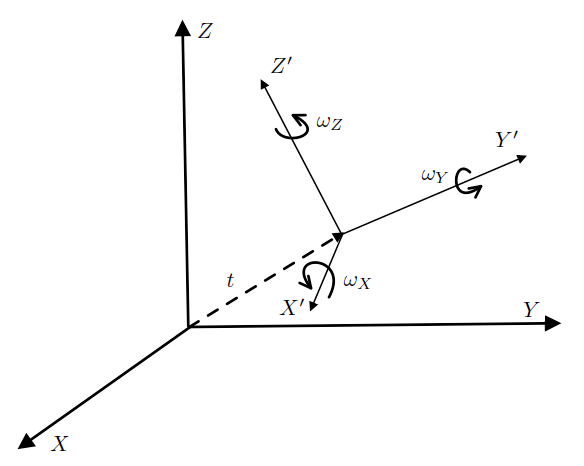
\includegraphics[width=0.5\linewidth]{images/figura1}
\end{center}
\caption{Coodenadas 3D, traslación y rotación}
\label{fig:figura1}
\end{figure}
Las dos transformaciones númeradas aquí se ven beneficiadas de la cualidad de la geometría proyectiva de operar con coordenadas homogéneas, lo cuál facilitará la resolución de las ecuaciones como se comenta en el siguiente punto.

\item \textbf{Coordenadas Homogéneas}\\
Las coordenadas homogéneas permiten combinar las transformaciones de rotación y translación en una única matriz. De esta manera, se consiguen expresiones compactas que posibilitan realizar los cálculos proyectivos de manera más eficiente.\\ 
En matemáticas, y de manera más concreta en el ámbito de la geometría proyectiva, las coordenadas homogéneas representan un instrumento fundamental para describir un punto en el espacio proyectivo. Dado el punto M de coordenadas cartesianas (X, Y, Z), se definen sus coordenadas homogéneas como (kX, kY, kZ, k), donde k es una constante distinta de cero. Para el caso particular de k = 0, dicho vector representa una dirección. La transformación entre ambos tipos de coordenadas es trivial y consiste en dividir los tres primeros términos de coordenadas homogéneas por el último.


\end{enumerate}
%%%%%%%%%%%%%%%%%%%%%%%%%%%%%%%%%%%%%%%%%%%%%%%%%%%%%%%%%%%%%%%%%%%%%%

\section{Aplicaciones en la realidad}

Una de las aplicaciones que podemos ver en la realidad de la geometría proyectiva es en el tratamiento de imágenes a través de una cámara, al pasar lo que capta del mundo real en 3D a una imagen en 2D.
Existen muchos modelos matemáticos que explican la geometría relativa a la proyección de una escena 3D sobre imagen 2D mediante una cámara. Uno de los más utilizados es el modelo ideal Pinhole y su variante con parámetros de distorsión. También veremos a continuación de estos modelos, un poco sobre calibración, muy necesaria para multitud de aplicaciones.
\begin{enumerate}

\item \textbf{Pinhole}\\
El modelo pinhole de una cámara consiste en un plano imagen R, lugar donde se proyecta la imagen y un punto C o centro óptico, lugar de convergencia del conjunto de rayos de dicha proyección. El parámetro f, o distancia focal, indica la distancia entre el plano imagen y el centro óptico.
\begin{figure}
\begin{center}
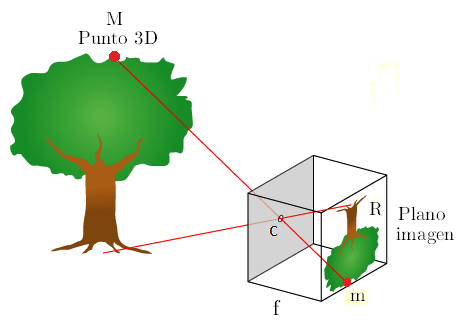
\includegraphics[width=0.6\linewidth]{images/pinhole}
\end{center}
\caption{Modelo de cámara Pinhole}
\label{fig:pinhole}
\end{figure}
Se puede observar como el punto 3D M se proyecta en el plano imagen formando el punto m (Fig. \ref{fig:pinhole}). Dicho punto se define como la recta que pasa por C y M. Aplicando el teorema de Thales podemos definir la relación entre las coordenadas no homogéneas de M y m:
\begin{figure}
\begin{center}
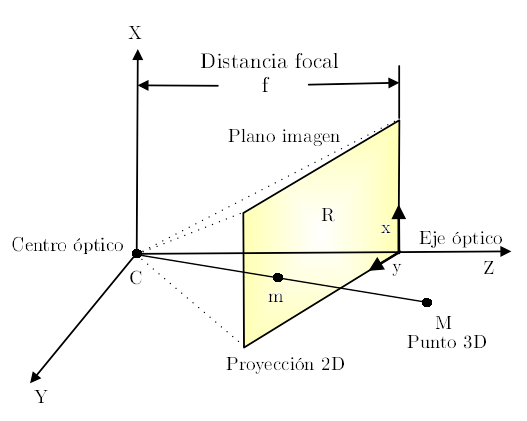
\includegraphics[width=0.7\linewidth]{images/pinholegeo}
\end{center}
\caption{Modelo geométrico equivalente a una cámara Pinhole}
\label{fig:pinholegeo}
\end{figure}
Suponiendo que dichas coordenadas son $ M =(X,Y,Z)^T $ y $ m=(x,y)^T $ obtenemos que, en coordenadas homogéneas:
\begin{equation}
Z\\
\begin{bmatrix}
x\\
y\\
1
\end{bmatrix}
=
\begin{bmatrix}
fX\\
fY\\
Z
\end{bmatrix}
=
\begin{bmatrix}
f & 0 & 0 & 0\\
0 & f & 0 & 0\\
0 & 0 & 1 & 0
\end{bmatrix}
\begin{bmatrix}
X\\
Y\\
Z\\
1
\end{bmatrix}
\end{equation}
y en forma matricial:
\begin{equation}
\lambda m = PM
\end{equation}
donde M y m representan las coordenadas homogéneas de esos mismos puntos. P es una matriz de dimensiones 3 x 4 conocida como matriz de proyección perspectiva de la cámara. El parámetro $ \lambda $ representa un factor de escala necesario para que se cumpla la igualdad, en este caso, igual a Z. Este factor representa una de las principales ventajas en el uso de coordenadas homogéneas en geometría proyectiva. Más información \cite{pinhole}

\item \textbf{Con distorsiones}\\
En este proceso de transformación del espacio 3D al plano imagen, se toma como referencia el sistema de la cámara. La transformación viene determinada por los parámetros intrínsecos, que representan las propiedades ópticas inherentes a la cámara. Se definen propiedades como:
\begin {itemize}
\item Coeficientes de distorsión : k1 y k2
\item Distancias focales (pixels no cuadrados en general): fx y fy
\item Desplazamiento, offset del centro de la imagen : Cx , Cy .
\end {itemize}
En principio, la imagen se forma según el modelo pinhole sin distorsión. Pero debido a que en la práctica, ninguna lente es perfecta, hay que tener en cuenta los tipos de distorsión que se pueden producir e intentar mitigarlos. Los dos tipos de distorsión más característicos son: distorsión radial, dada la forma de la lente, y distorsión tangencial producida por el ensamblado de las partes de la cámara. Estos modelos de distorsión conllevan una serie de operaciones en las que no vamos a entrar, pero de nuevo la geometría proyectiva ayuda en gran medida para simplificar cálculos.

En conclusión, la distorsión en la cámara se modela mediante seis coeficientes principalmente. Existen otro tipo de distorsiones, pero debido a que su impacto es reducido, no se suelen modelar.


\item \textbf{Calibración}\\
El proceso de calibración de una cámara consiste en determinar todos aquellos parámetros que intervienen en el proceso de formación de la imagen. En general, se definen dos tipos de parámetros: geométricos (disposición de los pixels en la imagen) y radiométricos, relativos al brillo del objeto proyectado. Tradicionalmente sólo se consideran los parámetros geométricos.

El proceso de calibración es fundamental para numerosas aplicaciones ya que posibilita determinar la correspondencia proyectiva entre un punto 3D en la escena y un punto 2D en el plano imagen. Por ejemplo:

Si el sistema de visión integrado no está correctamente calibrado, no dispondrá de información precisa sobre la posición relativa del objeto y por lo tanto será imposible manipularlo. Por otro lado, si la distorsión no se rectifica, los parámetros o características asociadas a dicho objeto, tales como la altura, área o perímetro serán corrompidas produciéndose errores de identificación y reconocimiento.\\
En el caso de la visión estéreo, en el que se realiza cierta triangulación para determinar la profundidad y así poder reconstruir la imagen 3D, la información acerca de las rectas de proyección de los pixels asociados en el par de imágenes ha de ser precisa. En este sentido, una cámara mal calibrada introduciría múltiples errores en el proceso de reconstrucción de la imagen.\\
En navegación pasiva se utiliza un conjunto de marcas sobre la imagen, en posiciones conocidas para determinar la posición relativa de la cámara, así como su orientación. Como cabe suponer, si existe un error en el calibrado, la navegación pasiva arrojaría resultados erróneos.\\
En ciertas aplicaciones tan sólo es necesario determinar la transformación proyectiva inversa. En otras, tan sólo la directa, como es el caso de predicción de un objeto en la imagen. En el caso particular de seguimiento o tracking donde se persigue estimar el posicionamiento continuo de un objeto móvil en la imagen, la transformación inversa permite situar el objeto (intersección plano y recta de proyección), mientras que la transformación directa avanza información sobre la posición futura del mismo.\\
Vista su importancia vamos a dar una breve definición de lo que es el proceso de calibración:\\
El proceso de calibración de una cámara tiene como objetivo determinar los parámetros de transformación entre los puntos 3D de la escena y la transformación proyectiva de dichos puntos sobre el espacio 2D imagen. Dicha transformación se rige por dos tipos de parámetros:
\begin {itemize}
\item Parámetros intrínsecos: Coeficientes de distorsión vistos anteriormente en el punto 2.
\item Parámetros extrínsecos: Conjunto de parámetros que determina la orientación y posición de la cámara en relación al sistema de coordenadas de referencia absoluto. Se definen como: Rotación, los ángulos $ \alpha ,\beta, \gamma$, y como Traslación, $ T_x, T_y, T_z $.
\end {itemize}
Una primera aproximación a la calibración nos llevaría a medir y almacenar los parámetros relativos a la recta de proyección asociados a cada pixel en la imagen, obteniendo como resultado una tabla inmensa. Ahora veremos que no es necesario, con métodos de calibración se puede llegar a obtener, interpolando y reduciendo el tamaño de la matriz, una precisión muy similar a la que se obtendría con la tabla completa.\\
Los métodos de calibración, seleccionan ciertos pixels de la imagen y calculan los parámetros relativos a la interpolación.Entre los algoritmos de calibrado más populares destaca el método de Tsai.

\underline{Método de Tsai}\\
Algoritmo propuesto por Roger Y. Tsai en 1987, es en la actualidad uno de los algoritmos de calibrado más popular e implementado. Sus principales características son las versatilidad y precisión. Está constituido por cuatro etapas cuyo resultado final es la transformación del punto 3D al plano imagen.
\begin{enumerate}
\item Transformación del sistema de coordenadas de la escena al de la cámara. Primero se produce la transformación de rotación y posteriormente la de translación, en ese orden.
\item Transformación del sistema de coordenadas de la cámara 3D al mundo de las coordenadas ideales, libres de distorsión en el plano imagen según el modelo pinhole. La distancia focal f es el parámetro a calibrar.
\item Transformación del sistema de coordenadas de la imagen ideal al sistema de coordenadas distorsionado en el sensor. En este caso, el parámetro a calibrar es K1 ya que K2 se considera despreciable.
\item Transformación del sistema de coordenadas de la imagen con distorsión (xd , yd ) al sistema de coordenadas en el computador (xf , yf ).\\
Para más información, ver \cite{tsai}. 
\end{enumerate}
\end {enumerate}

%%%%%%%%%%%%%%%%%%%%%%%%%%%%%%%%%%%%%%%%%%%%%%%%%%%%%%%%%%%%%%%%%%%%%

\section{Conclusión}




\bibliographystyle{plain}
\bibliography{refs}

\end{document}
